\chapter{序論}

\section{研究背景}
スマートタグとは貴重品などに取り付け, 紛失した際に捜索を補助するデバイスである. 
補助の方法はタグが音を鳴らす方法と付近のスマートフォンと無線通信する方法が一般的である. 
近年こうした製品が普及しており, なくしものの対策に需要があることを示唆している. 
しかし特性上タグの取り付けが困難な物もある. 
例えば入れ歯は口内で使用するために衛生や防水, 日常生活の邪魔になるなどの理由で取り付けが難しい. 

\section{関連研究}
タグを必要としないなくしもの対策として, 草野\index{くさの@草野}らが提案する家庭内での移動マニピュレータによるベイズ推定と自然言語処理を用いた物品捜索手法\cite{kusano}がある. 
この手法ではまず捜索範囲をいくつかのエリアに区切る. 
そして各エリアごとに過去そのエリアを捜索し捜索対象を発見した回数$\alpha$, 発見できなかった回数$\beta$を用い, 
捜索対象の存在確率を$ \alpha / (\alpha + \beta)$と定義し, 存在確率が最大のエリアを捜索する. 
また存在確率が最大のエリアが複数ある場合は移動マニピュレータが位置するエリアからの距離, ならびに自然言語処理によるエリア内の家具の名前と捜索対象の名前の類似度も考慮する. 

\begin{figure}[H]
    \begin{center}
        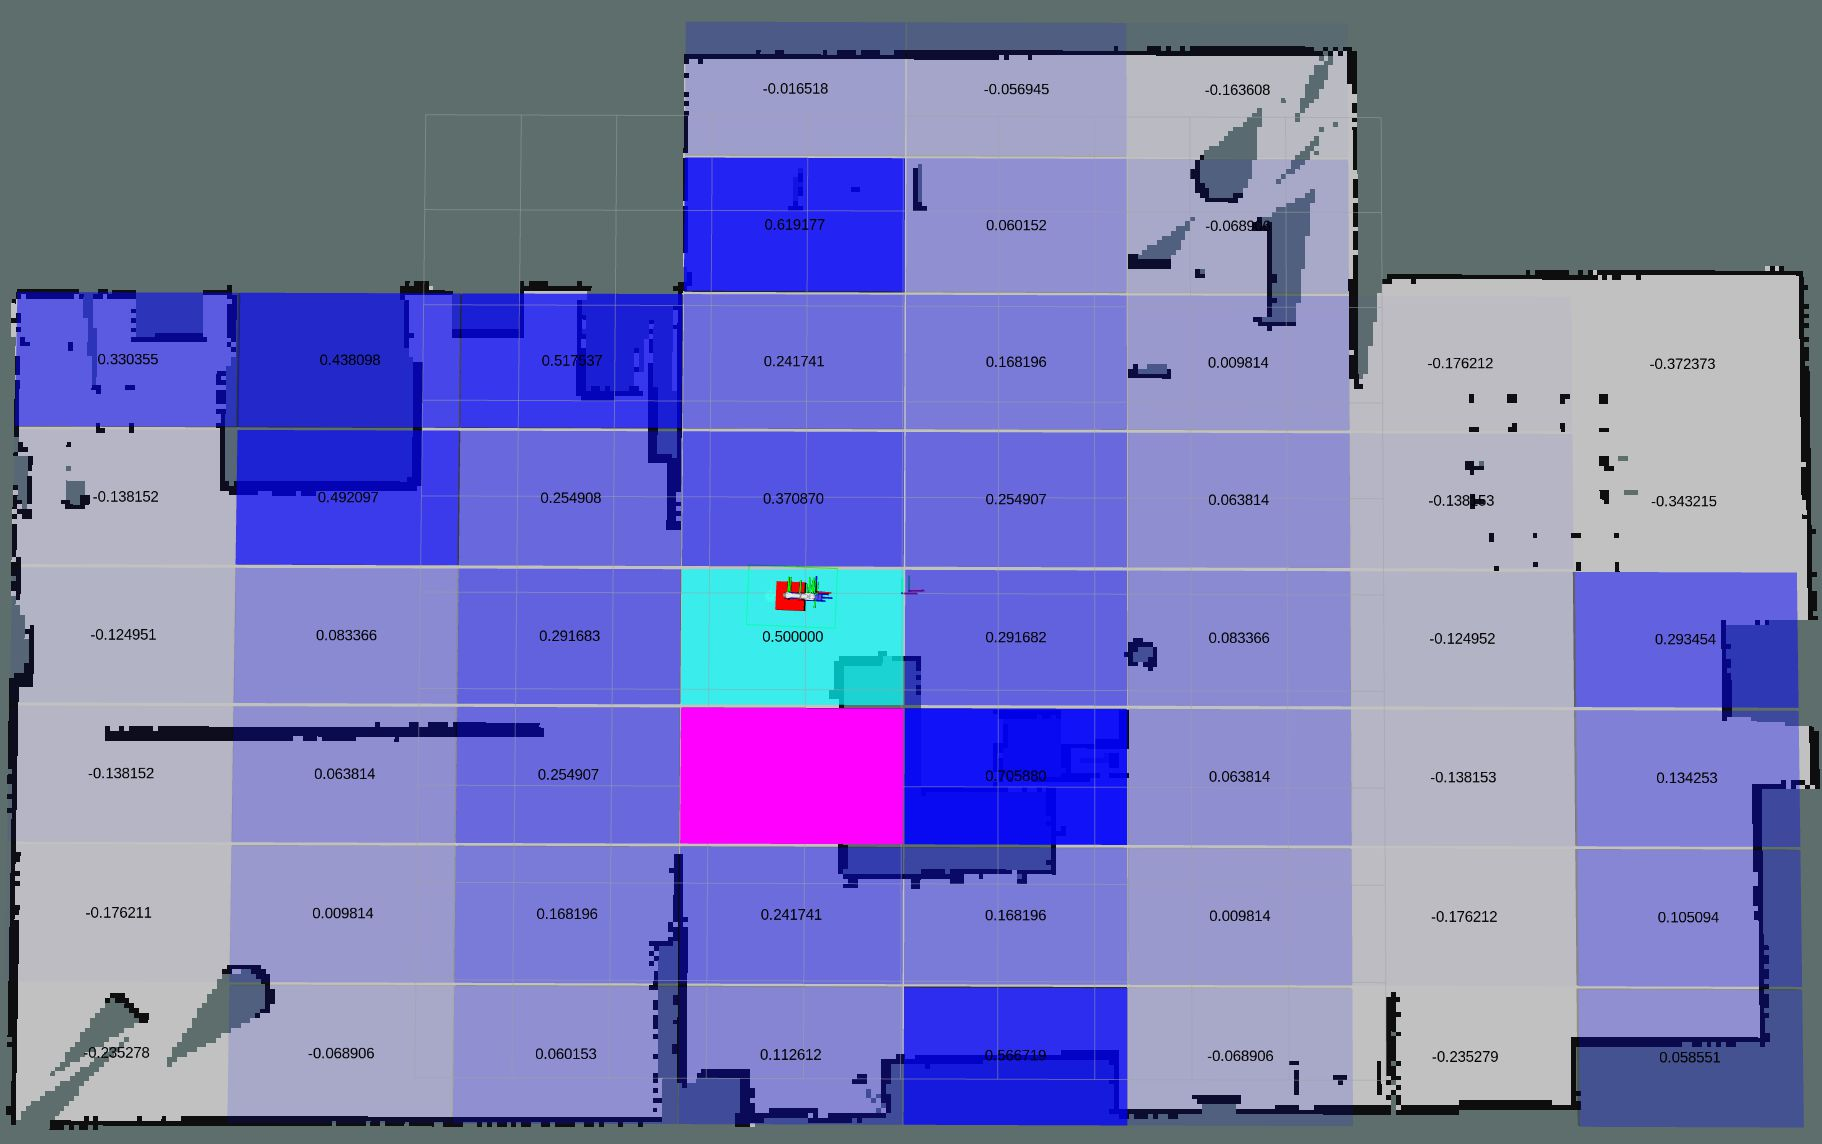
\includegraphics[width=0.8\linewidth]{figs/kusano.jpg}
        \caption{Existence probability of target object}
        \label{fig:kusano}
    \end{center}
\end{figure}

この手法は捜索する主体が移動マニピュレータであることを前提としている. 
しかし現在, そうしたロボットはスマートタグの代替としては高価であり利用できる環境は限定される. 

また, 人がなくしものを捜索する際に捜索対象の所有者(以下, 単に所有者という)がよく使う場所を重点的に捜索する等, 所有者の行動を手がかりにする. 
一方この手法の場合, なくしものは発生頻度が高くないため$\alpha$が同じエリアが複数ある状況が長く続くことが想定される. 
こうした状況ではエリア間の距離と単語の類似度を重視することになるが, これらは所有者の行動を反映していない. 

\section{研究目的}
なくしものの捜索をなくしものがある場所を予測する部分と予測した場所に移動し周辺を見回すという部分に分解して考える. 
草野らの手法は双方が密接に結びついているために移動マニピュレータが必要となる. 
そこで本研究は移動等の部分は扱わず, なくしものの位置を推定する手法を提案する. 
位置推定にあたり所有者の行動を反映するため, なくしものが発生するまでの過程を確率論を用いてモデル化する. 
また提案手法の有効性を確認する準備として, なくしものの位置を推定するソフトウェアと推定に用いるパラメータの機械学習のためのシステムの開発も行う. 
